\section{Resultate}

		Wir haben verschiedene Fl�chen mit verschiedenen Aufl�sungen berechnet. Je nach Ausgangsbild ist die Superposition mehr oder weniger gut erkennbar. Wie in \fref{sec:geeignetesF} erw�hnt, hat sich eine Spirale von Punkten bew�hrt, die wir hier anhand vier verschiedenen Schritten zeigen wollen. Das erste Bild ist jeweils die Fl�che $f$ f�r den jeweiligen Schritt, alle Punkte haben das selbe Potential. Pro Bild f�hrten wir 180\,000 Iterationen durch.
	

	\newlength\breite
	\setlength\breite{8cm}
	\begin{figure}[h]
			\centering
		\begin{tabular}{cc}
			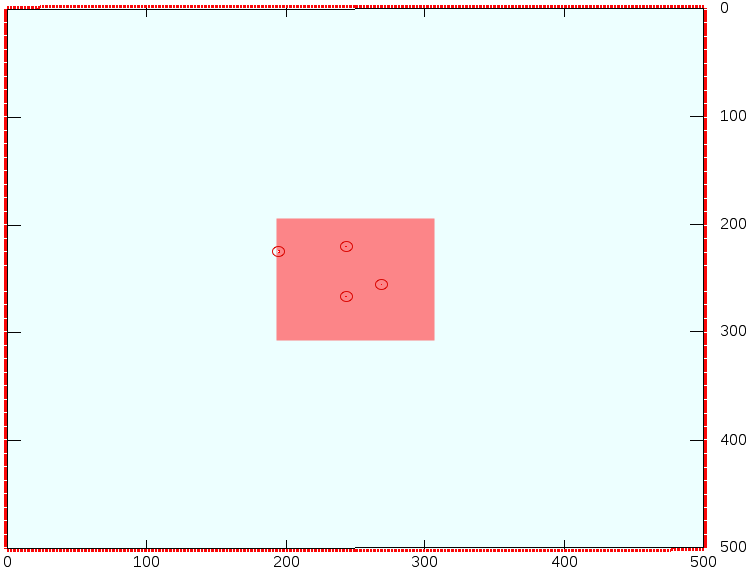
\includegraphics[width=\breite]{./images/resultate/grfl/step0057.png}
			& 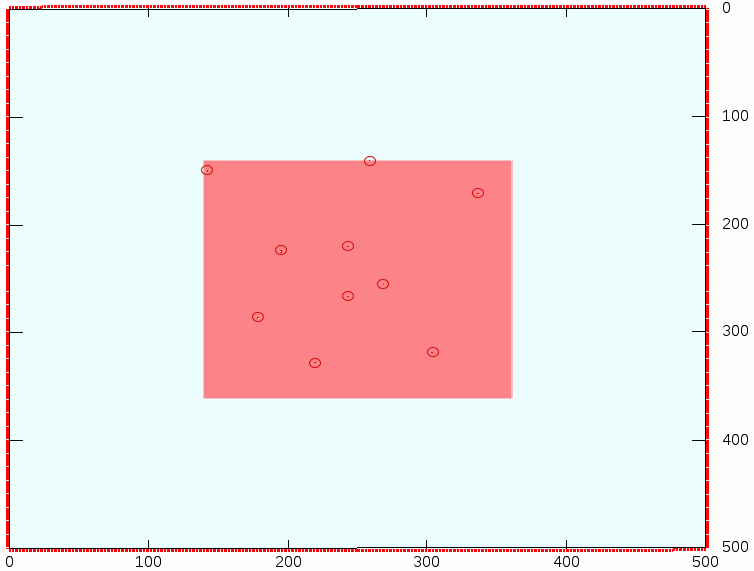
\includegraphics[width=\breite]{./images/resultate/grfl/step0111.png}\vspace{1cm}\\
			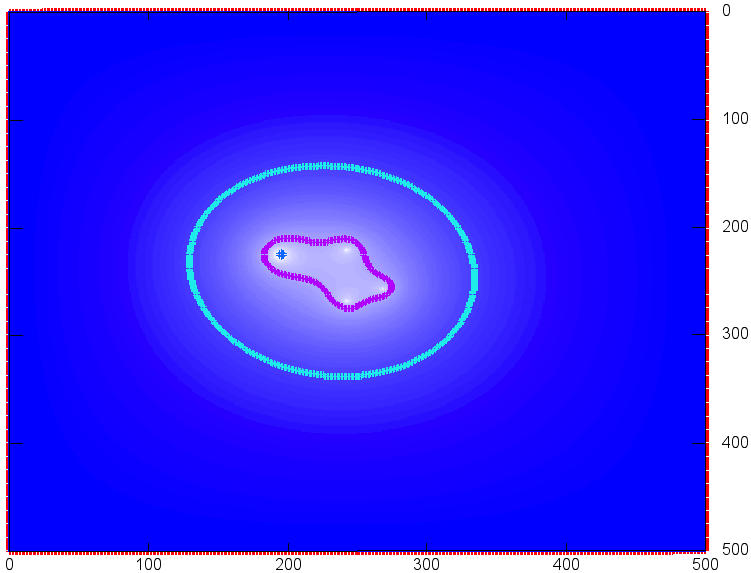
\includegraphics[width=\breite]{./images/resultate/cp/step0057.png}
			& 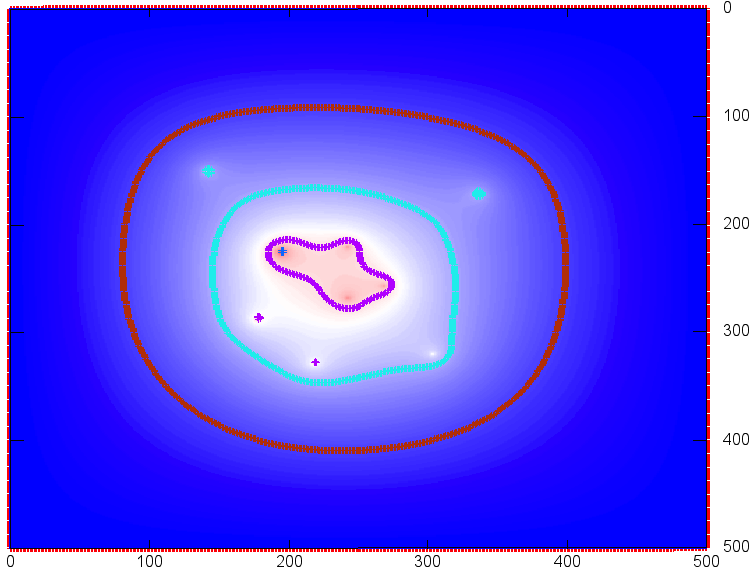
\includegraphics[width=\breite]{./images/resultate/cp/step0111.png}\vspace{1cm}\\
			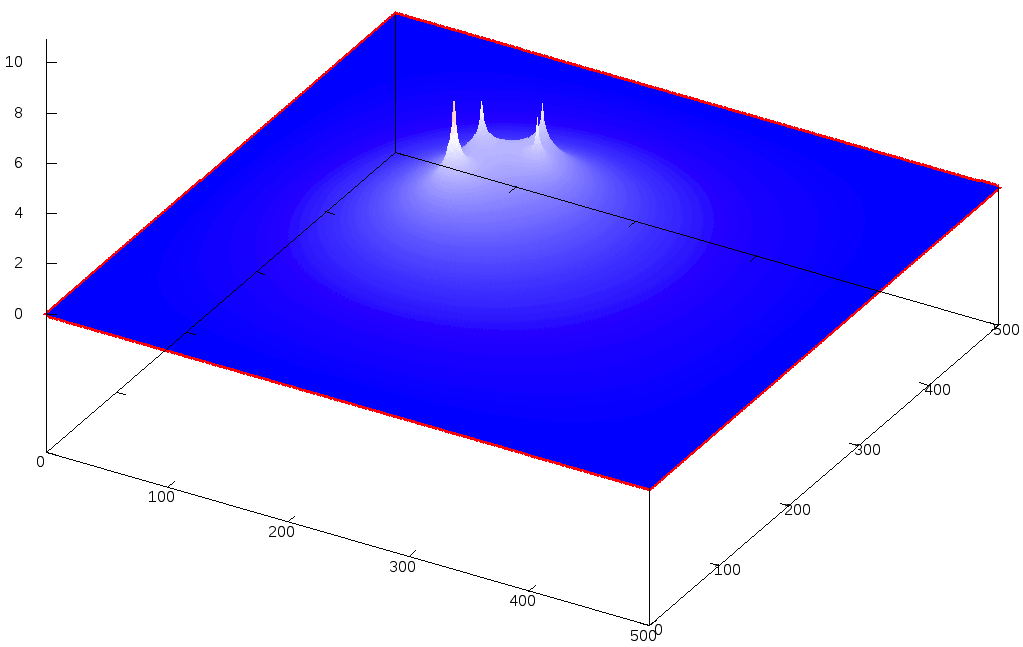
\includegraphics[width=\breite]{./images/resultate/np/step0057.png}
			& 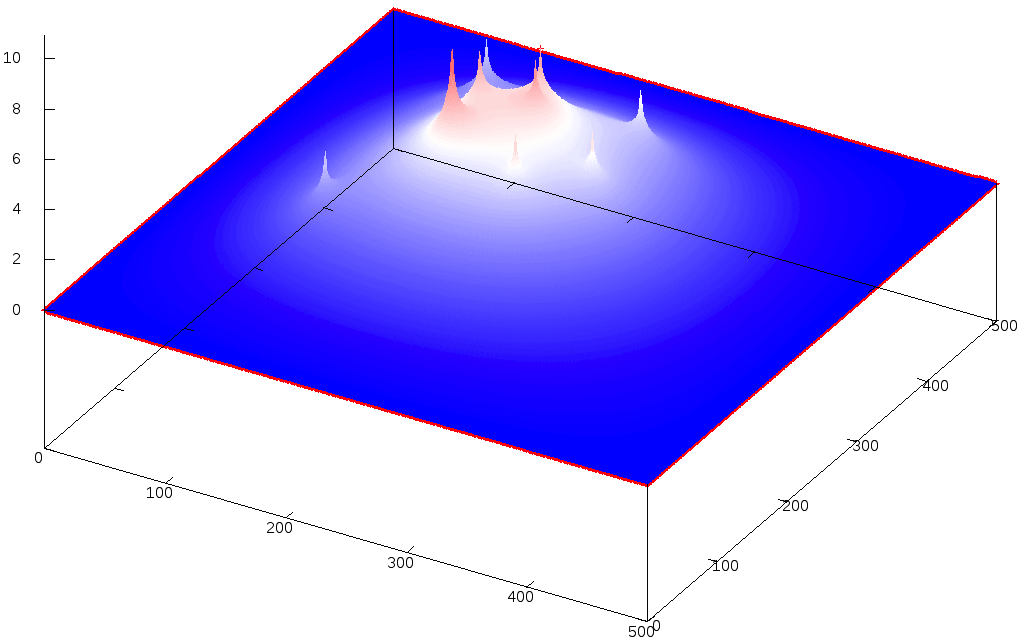
\includegraphics[width=\breite]{./images/resultate/np/step0111.png}
		\end{tabular}		
			\caption{Visualisierung von Green's Function: Schritte 75 und 111 }
	\end{figure}
	
	\begin{figure}[h]
			\centering
		\begin{tabular}{cc}
			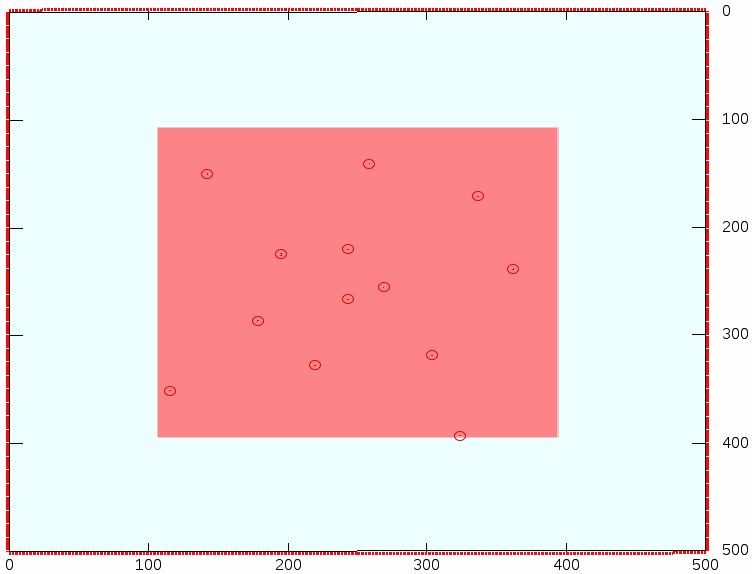
\includegraphics[width=\breite]{./images/resultate/grfl/step0144.png}
			& 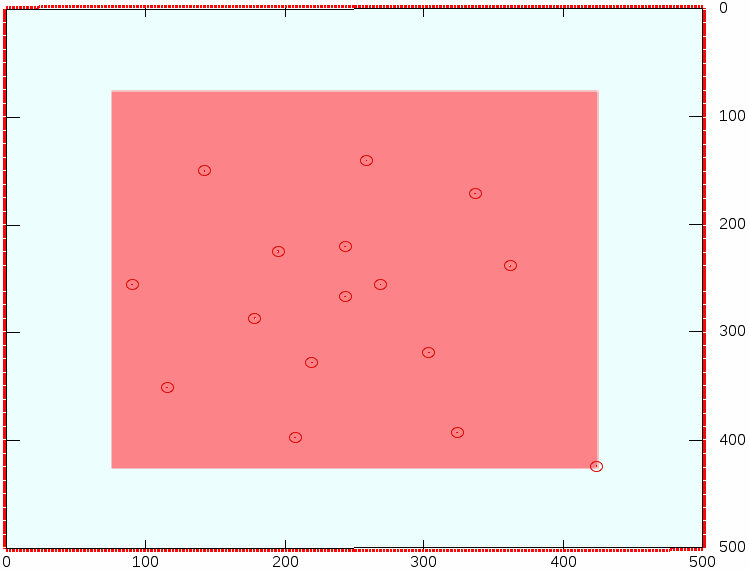
\includegraphics[width=\breite]{./images/resultate/grfl/step0175.png}\vspace{1cm}\\
			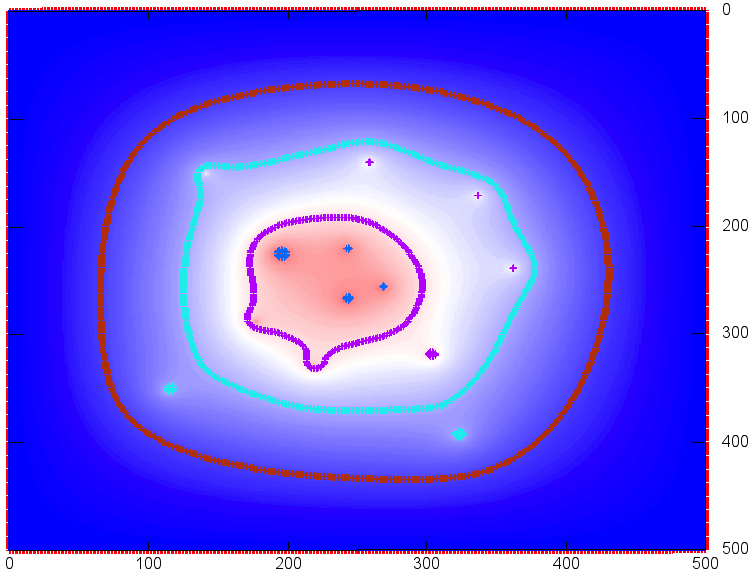
\includegraphics[width=\breite]{./images/resultate/cp/step0144.png}
			& 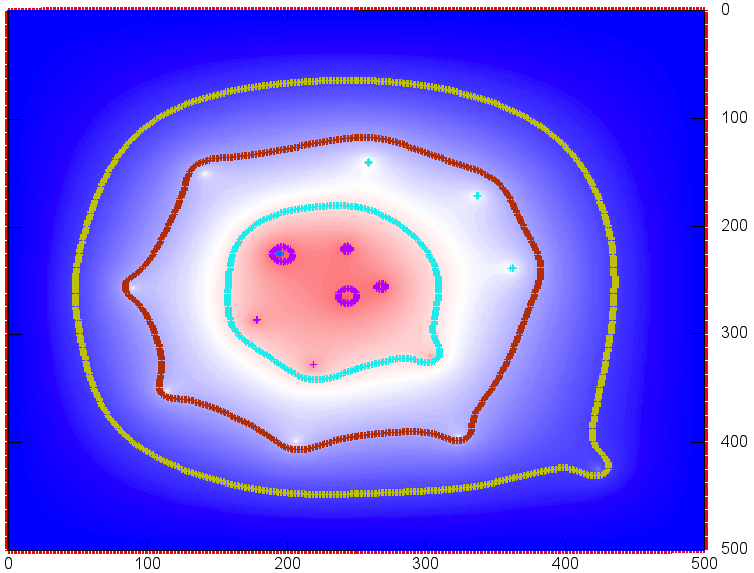
\includegraphics[width=\breite]{./images/resultate/cp/step0175.png}\vspace{1cm}\\
			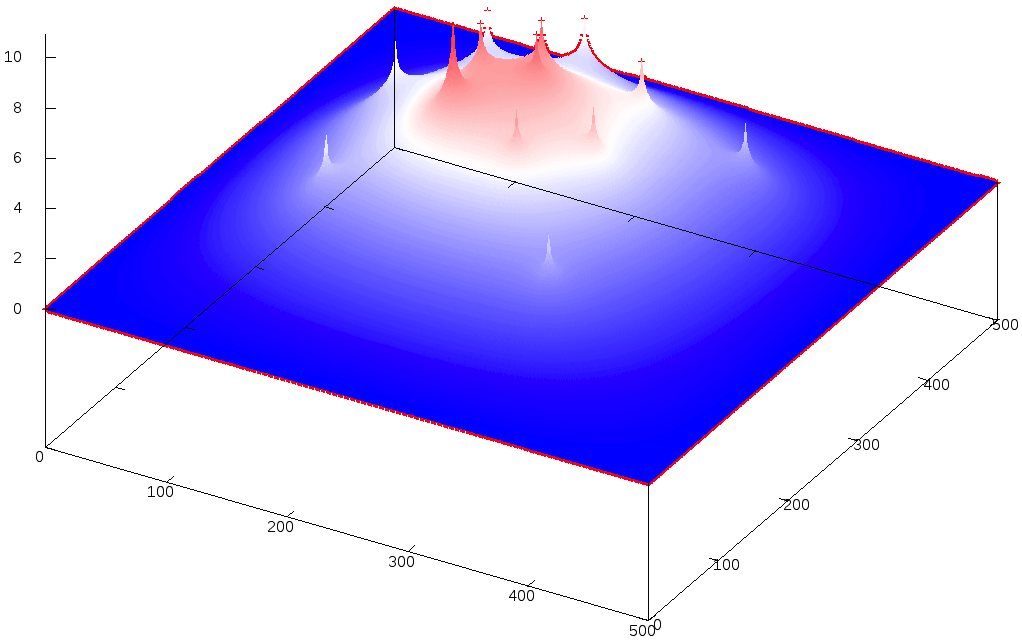
\includegraphics[width=\breite]{./images/resultate/np/step0144.png}
			& 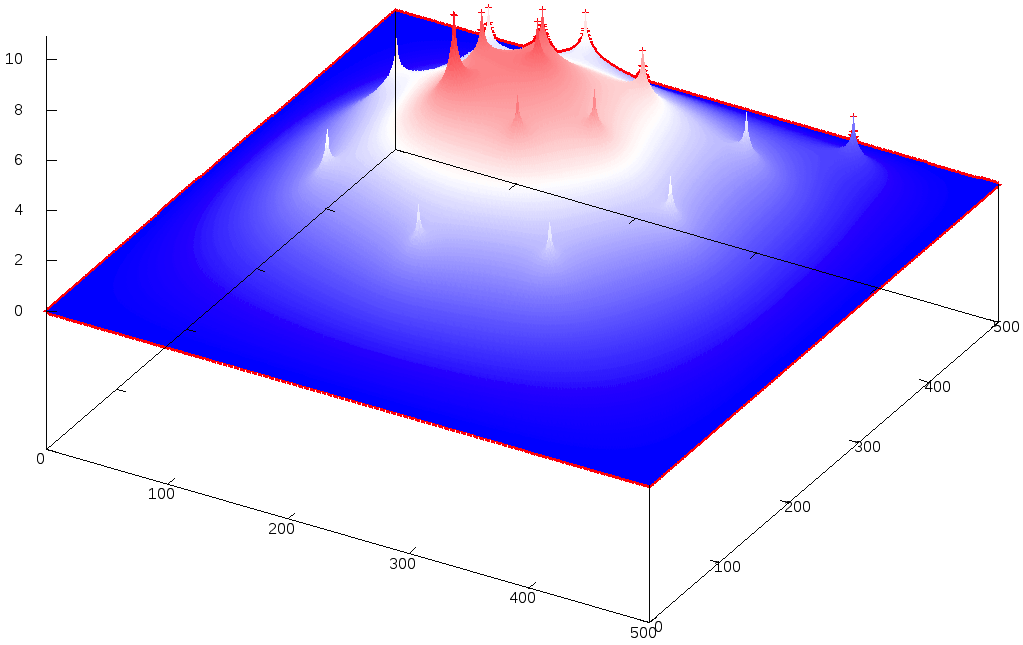
\includegraphics[width=\breite]{./images/resultate/np/step0175.png}
		\end{tabular}		
			\caption{Visualisierung von Green's Function: Schritte 144 und 175 }
	\end{figure}